% chapter02.tex

 %%%%%%%%%%%%%%%%%%%%%%%%%%%%%%%%%%%%%%%%%%%%%%%%%%%%%%%%%%%%%%%%%%%%%%%%%%%%%
 %                                                                           %
 %    PyMS documentation                                                     %
 %    Copyright (C) 2005-8 Vladimir Likic                                    %
 %                                                                           %
 %    The files in this directory provided under the Creative Commons        %
 %    Attribution-NonCommercial-NoDerivs 2.1 Australia license               %
 %    http://creativecommons.org/licenses/by-nc-nd/2.1/au/                   %
 %    See the file license.txt                                               %
 %                                                                           %
 %%%%%%%%%%%%%%%%%%%%%%%%%%%%%%%%%%%%%%%%%%%%%%%%%%%%%%%%%%%%%%%%%%%%%%%%%%%%%

\chapter{GC-MS Data Model}

PyMS can read gas chromatography-mass spectrometry (GC-MS) data stored in
Analytical Data Interchange for Mass Spectrometry (ANDI-MS),\footnote{ANDI-MS
was developed by the Analytical Instrument Association.} and Joint Committee on
Atomic and Molecular Physical Data (JCAMP-DX)\footnote{JCAMP-DX is maintained by
the International Union of Pure and Applied Chemistry.} formats. These formats
are essentially recommendations, and it is up to individual vendors of mass
spectrometry processing software to implement ``export to ANDI-MS'' or ``export
to JCAMP-DX'' features in their software. It is also possible to get third party
converters. The information contained in the exported data files
can vary significantly, depending on the instrument, vendor's software, or
conversion utility.

For PyMS, the minimum set of assumptions about the information contained in the
data file are:
\begin{itemize}
    \item The data contain the mz and intensity value pairs across a scan.
    \item Each scan has a retention time.
\end{itemize}

Internally, PyMS stores the raw data from ANDI files or JCAMP files as a
GCMS\_data object. Once a GCMS\_data object has been created, the raw data can
not be modified. The operations (methods) available are illustrated in the
following sections.

\section{Reading GCMS data}

This section demonstrates the GCMS data reading functions of PyMS in a tutorial
like manner. The data files used in the examples are provided in the project
`pyms2-data'. The commands executed interactively are grouped together by
example, and provided as Python scripts in the project `pyms2-test'.

The setup used in the examples below is as follows. The projects `pyms2',
`pyms2-test', `pyms2-docs', and `pyms2-data' are all in the same directory. In
the project `pyms2-test' there is a directory corresponding to each example
coded with the example number (ie. {\tt pyms2-test/01a/} corresponds to Example
1a). In each example directory, there is a script named `proc.py' which contains
the commands given in the example. Provided that the paths to `pyms2' and
`pyms2-data' are set properly, these scripts could be run with the following
command:

\begin{verbatim}
$ python proc.py
\end{verbatim}

Before running each example the Python interpreter was made aware of the
PyMS location with the following commands:

\begin{verbatim}
import sys
sys.path.append("../../pyms2")
\end{verbatim}

For brevity these commands will not be shown in the examples below, but
they are included in `pyms2-test' example scripts.  The above path may need
to be adjusted to match your own directory structure.

All data files (raw data files, peak lists etc.) used in the example below
can be found in `pyms2-data'.

\subsection{Reading JCAMP GC-MS data into PyMS}

\noindent
[ {\em This example is in pyms2-test/01a} ]

The PyMS2 package pyms2.GCMS.IO.JCAMP provides capabilities to read the raw
GC-MS data stored in the JCAMP-DX format.

The file `gc01\_0812\_066.jdx' (located in `pyms2-data') is a GC-MS experiment
converted from Agilent ChemStation format to JCAMP format using File Translator
Pro.\footnote{ChemSW, Inc.} This file can be loaded in Python as follows:

\begin{verbatim}
>>> from pyms2.GCMS.IO.JCAMP.Class import JCAMP_reader
>>> jcamp_file = "../../pyms2-data/gc01_0812_066.jdx"
>>> data = JCAMP_reader(jcamp_file)
 -> Reading JCAMP file '../../pyms2-data/gc01_0812_066.jdx'
>>>
\end{verbatim}

\noindent
The above command creates the object `data' which is an {\em instance}
of the class GCMS.IO.JCAMP\_reader.

\subsection{Reading ANDI GC-MS data into PyMS}

\noindent
[ {\em This example is in pyms2-test/01b} ]

The PyMS2 package pyms2.GCMS.IO.ANDI provides capabilities to read the raw
GC-MS data stored in the ANDI-MS format.

The file `gc01\_0812\_066.cdf' (located in `pyms2-data') is a GC-MS experiment
converted to ANDI-MS format from Agilent ChemStation (from the same data as in
example 01a above). This file can be loaded as follows:

\begin{verbatim}
>>> from pyms2.GCMS.IO.ANDI.Class import ANDI_reader
>>> ANDI_file = "../../pyms2-data/gc01_0812_066.cdf"
>>> data = ANDI_reader(ANDI_file)
 -> Reading netCDF file '../../pyms2-data/gc01_0812_066.cdf'
>>>
\end{verbatim}

\noindent
The above command creates the object `data' which is an {\em instance}
of the class GCMS.IO.ANDI\_reader.

\subsection{Exploring a GCMS data object}

\noindent
[ {\em The following examples are in pyms2-test/01a and pyms2-test/01b} ]

The object `data' (from the two previous examples) stores the raw data as a {\em
GCMS\_data} object. The data and properties of the GCMS\_data object can be
accessed by the following:

\begin{verbatim}
>>> gcms_data = data.get_gcms_data()
\end{verbatim}

Within the GCMS\_data object, raw data are stored as a list of {\em Scan}
objects and a list of retention times.  There are several methods available to
access data and attributes of the GCMS\_data and Scan objects.

The GCMS\_data object methods relate to the raw data. The main properties
relate to the masses, retention times and scans. For example, the
minimum and maximum mass from all of the raw data can be returned by the
following:

\begin{verbatim}
>>> gcms_data.get_min_mass()
>>> gcms_data.get_max_mass()
\end{verbatim}

A list of all retention times can be returned by:

\begin{verbatim}
>>> time = gcms_data.get_time_list()
\end{verbatim}

The index of a specific retention time (in seconds) can returned by:

\begin{verbatim}
>>> gcms_data.get_index_at_time(400.0)
\end{verbatim}

\noindent
Note that this returns the index of the retention time in the
data closest to the given retention time (400.0 seconds).

The method {\tt get\_tic()} returns a total ion chromatogram (TIC) of the data
as an IonChromatogram object:

\begin{verbatim}
tic = gcms_data.get_tic()
\end{verbatim}

\noindent
The IonChromatogram object is covered in a later section.

A list of all the raw Scan objects can be returned by:

\begin{verbatim}
>>> scans = gcms_data.get_scan_list()
\end{verbatim}

\noindent
The Scan object has methods relating to an individual scan. This is covered in
the next section.

\subsection {Exploring a Scan data object}

\noindent
[ {\em The following examples are in pyms2-test/01a and pyms2-test/01b} ]

A Scan object contains a list of masses and a corresponding list of intensity
values from a single mass-spectrum scan.

A list of all masses in a scan (e.g. the 1st scan) is returned by:

\begin{verbatim}
>>> scans[0].get_mass_list()
\end{verbatim}

A list of all corresponding intensities in a scan is returned by:

\begin{verbatim}
>>> scans[0].get_intensity_list()
\end{verbatim}

The maximum and minimum mass in an individual scan (e.g. the 1st scan) are
returned by:

\begin{verbatim}
>>> scans[0].get_min_mass()
>>> scans[0].get_max_mass()
\end{verbatim}





% %%%%%%%%%%%%%%%%%%%%%%%%%%%%%%%%%%%%%%%%%%%%%%%%%%%%%%%%%%%%%%%%%
% \chapter{Intensity Matrix}
% Each scan only
% contains information about the mass/charge and intensity at intensity peaks in
% the scan. This means that consecutive scans do not necessarily contain the
%same
% mass/charge values. For data processing, it is often necessary to convert the
% data to a matrix with a set number of mass/charge values and number of scans.
% This means some mechanism for converting mass/charge values to a set of fixed
% values is required. In PyMS there are functions to explicitly handle the
% conversion of mass/charge values to consistent values across all scans.
%
% The general scheme for converting mass/charge values is to bin intensity
% values
% based on the interval the corresponding mass/charge values belongs to. The
% general procedure is
% as follows:
% \begin{itemize}
%     \item for a given bin size
%     \item determine the maximum and minimum mass/charge values in entire data
%set.
%     \item calculate the number of bins in the total mass/charge range.
%     \item centre the first bin at the minimum mass/charge value.
%     \item sum intensities corresponding to all mass/charge values that are in
%a
% given bin.
% \end{itemize}
%
% A specific function to round mass/charge values is also available. The
% process is that all intensity values for a mass/charge values that fall within
%a
% unit width about each given integer value are added together. In PyMS, a
% mass/charge is considered to belong to a bin when it is equal to or greater
% than half the bin width from the centre of the bin, and less than half the bin
% width from the centre of the bin.
% %That is, a mass/charge, $m$ is considered to belong to a bin when $c-w/2\le
% %m\lt c+w/2$, where $c$ is the centre of the bin, and $w$ is the width of the
% %bin.
%
% Figure~\ref{fig:binning} illustrates the process of assigning bins to the
% mass/charge axis and summing all intensities in a given bin. The result is a
% new mass/charge axis with mass/charge values corresponding to the centre of
% each bin.
%
% \begin{figure}[htp]
% \begin{center}
% \includegraphics{graphics/binning/binning.eps}
% \caption{Mass/charge intensity values are added to bins based on a pre-set bin
% size and the minimum mass/charge value of all the scan data. All intensities
%in
% a given bin width (top) are added and given a mass/charge value of the centre
% of the bin (bottom). For integer binning, each bin has a width of one and is
% centred at integer values.}
% \label{fig:binning}
% \end{center}
% \end{figure}
%
% %%%%%%%%%%%%%%%%%%%%%%%%%%%%%%%%%%%%%%%%%%%%%%%%%%%
% \noindent
% An IonChromatogram object is a one dimensional vector containing
% mass intensities as a function of retention time. This can can be either
% m/z channel intensities (for example, ion chromatograms at m/z = 65),
% or cumulative intensities over all measured m/z (TIC).
%
% An ion chromatogram object has a method {\tt is\_tic()} which returns
% True is the ion chromatogram is TIC, False otherwise:
%
% \begin{verbatim}
% >>> print "'tic' is a TIC:", tic.is_tic()
% 'tic' is a TIC: True
% >>> print "'ic' is a TIC:",ic.is_tic()
% 'ic' is a TIC: False
% \end{verbatim}
%
% \subsection{Writing data to a file}
%
% The method {\tt write()} of IonChromatogram object allows one to save
% the ion chromatogram object to a file:
%
% \begin{verbatim}
% >>> tic.write("output/tic.dat", minutes=True)
% >>> ic.write("output/ic.dat", minutes=True)
% \end{verbatim}
%
% \noindent
% The flag minutes=True indicates that retention time will be saved in minutes.
% The ion chromatogram object saved with with the {\tt write{}} method is a
% plain ASCII file which contains a pair of (retention time, intensity) per
% line:
%
% \begin{verbatim}
% $ head tic.dat
%   5.0944      745997.0000
%   5.1002      726566.0000
%   5.1059      717704.0000
%   5.1116      684214.0000
%   5.1173      701866.0000
%   5.1230      893306.0000
%   5.1287     1278099.0000
%   5.1345     1290984.0000
%   5.1402      925558.0000
%   5.1459      644122.0000
% \end{verbatim}
%
% \noindent
% Figure \ref{fig:tic-plot} shows the plot of the file 'tic.dat' produced with
%the
% program Gnuplot. The Gnuplot script used to produce this plot is provided
% as pyms-test/01/output/plot.gnu.
%
% \begin{figure}[htp]
% \begin{center}
% %x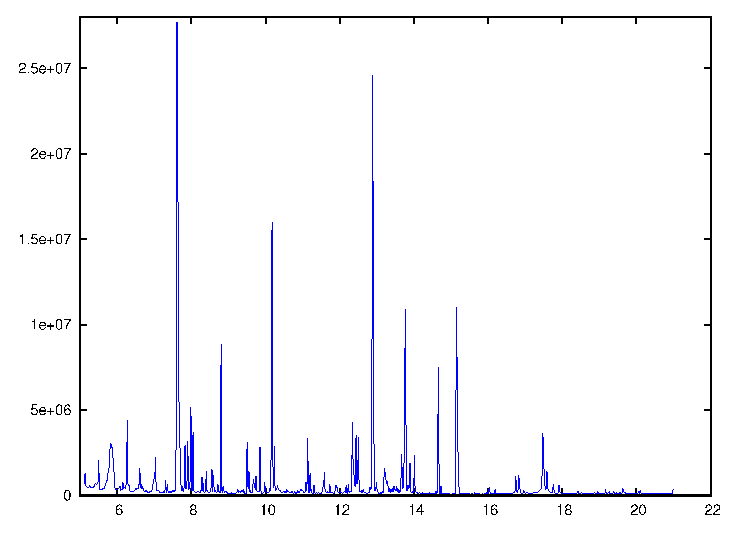
\includegraphics{graphics/pyms-test/tic.eps}
% \caption{The Gnuplot plot of the file 'tic.dat'}
% \label{fig:tic-plot}
% \end{center}
% \end{figure}
